\label{section:1d_column_example}
This example can be found in the folder \verb+MUT_Examples\1_VSF_Column+
\begin{verbatim}
! Examples\1_VSF_Column:
!   A modflow project of a 1D column generated from a simple 2d rectangular mesh
build modflow usg
\end{verbatim}
The template mesh is generated using the following instructions:
\begin{verbatim}
    generate uniform rectangles
    1.0, 1   !  Mesh length in X-direction and number of rectangular elements
    1.0, 1   !  Mesh length in Y-direction and number of rectangular elements
\end{verbatim}


The 1D column example uses a single 1m X 1m rectangular element as the template mesh for building the GWF domain.
    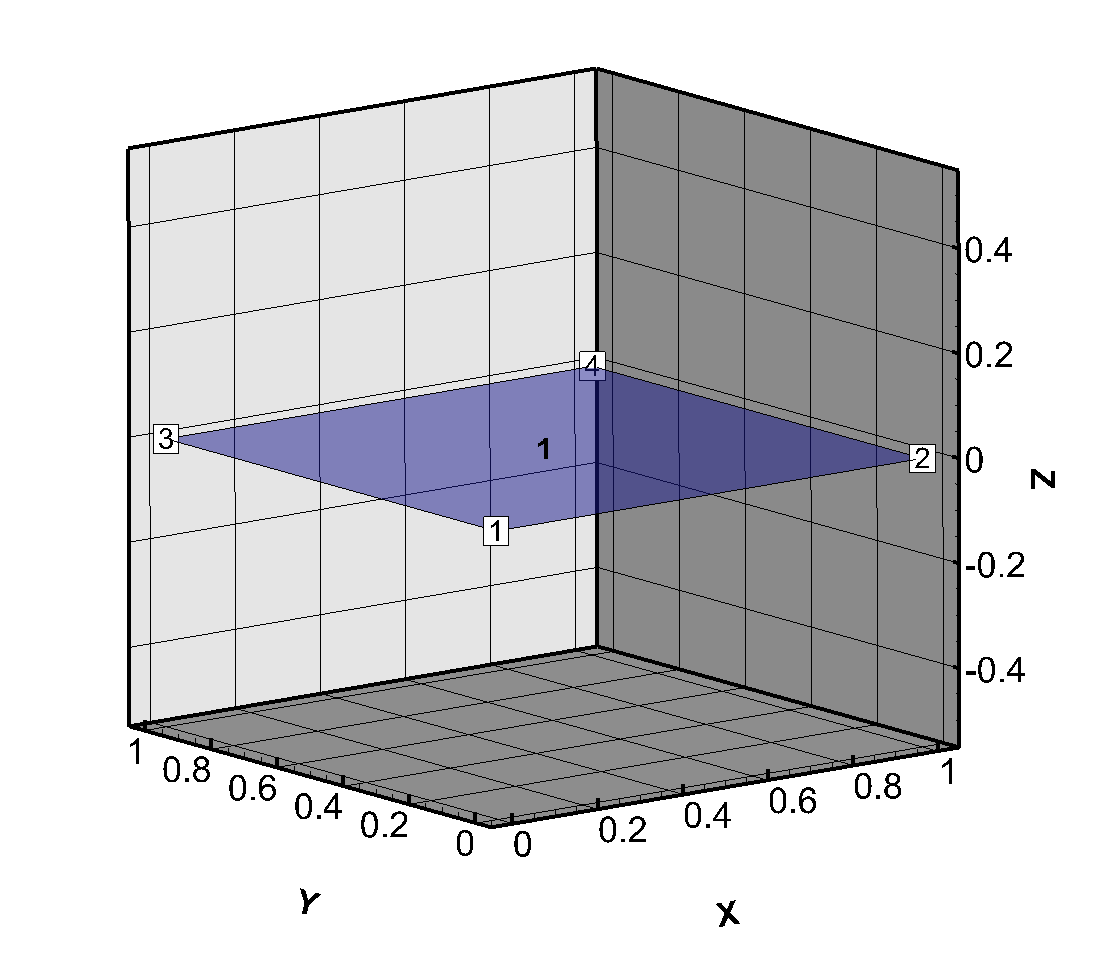
\includegraphics[width=0.6\textwidth]{column_template}



Figure~\ref{fig:1D_Build} shows the The 1D column example uses a single 1 m by 1 m rectangular element as the template mesh for building the GWF domain.
\begin{figure}
    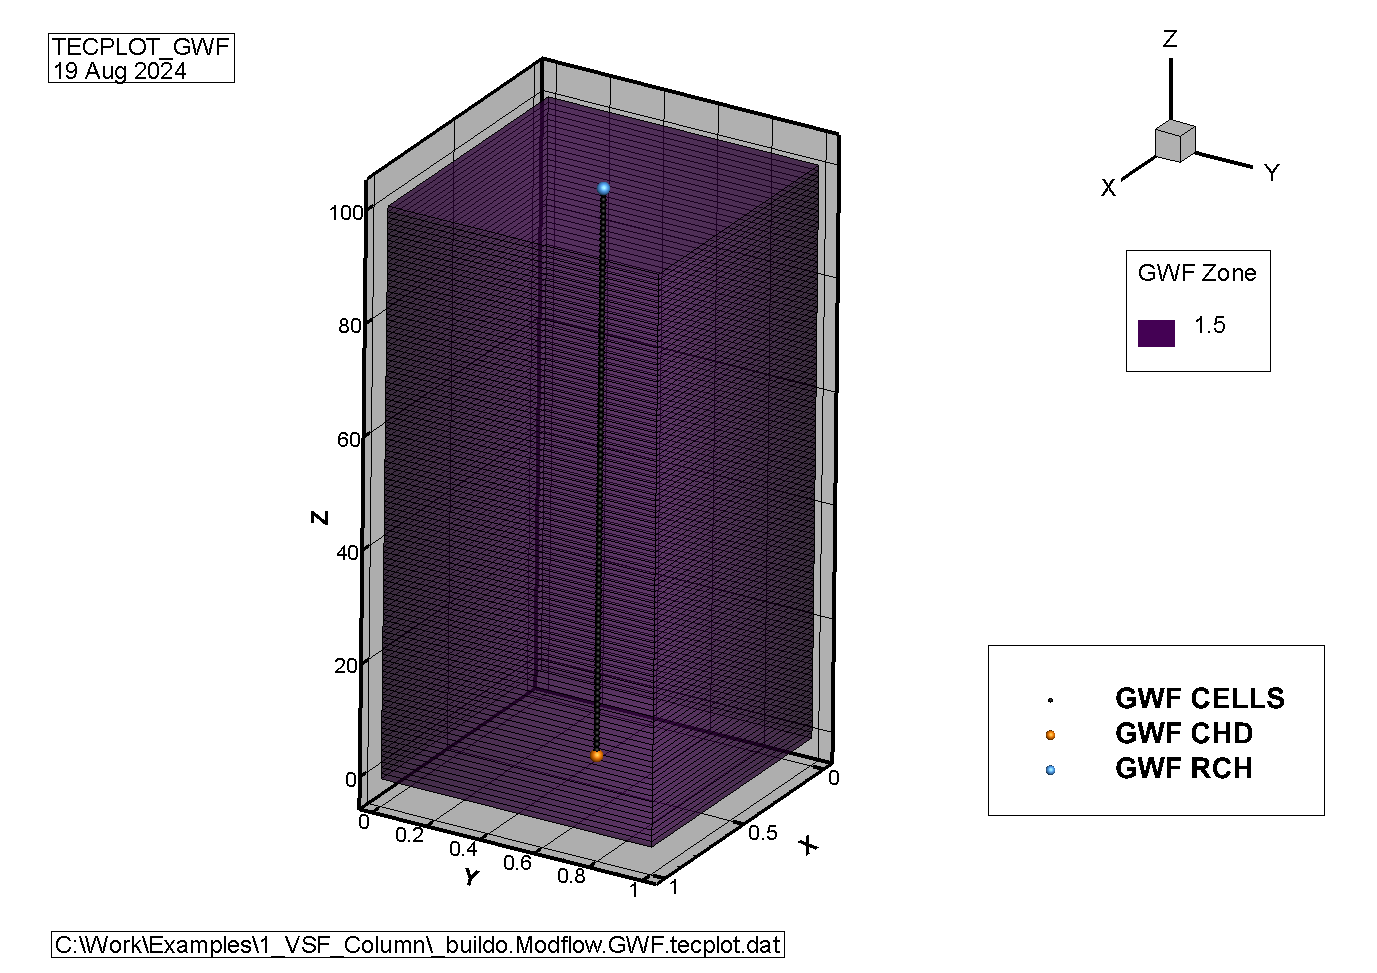
\includegraphics[width=0.9\textwidth]{column_build}
    \caption{1D column build} \label{fig:1D_Build}
\end{figure}
